%
% konstruktion.tex
%
% (c) 2021 Prof Dr Andreas Müller, OST Ostschweizer Fachhochschule
%
\begin{frame}[t]
\frametitle{Konstruktion mit Zirkel und Lineal}
\vspace{-20pt}
\begin{columns}[t,onlytextwidth]
\begin{column}{0.48\textwidth}
\begin{block}{Strahlensatz}
\uncover<6->{%
Jedes beliebige rationale Streckenverhältnis $\frac{p}{q}$
kann mit Zirkel und Lineal konstruiert werden.}
\end{block}
\end{column}
\begin{column}{0.48\textwidth}
\uncover<7->{%
\begin{block}{Kreis--Gerade}
Aus $c$ und $a$ konstruiere $b=\sqrt{c^2-a^2}$
\uncover<13->{%
$\Rightarrow$ jede beliebige Quadratwurzel kann konstruiert werden}
\end{block}}
\end{column}
\end{columns}
\begin{columns}[t,onlytextwidth]
\begin{column}{0.48\textwidth}
\begin{center}
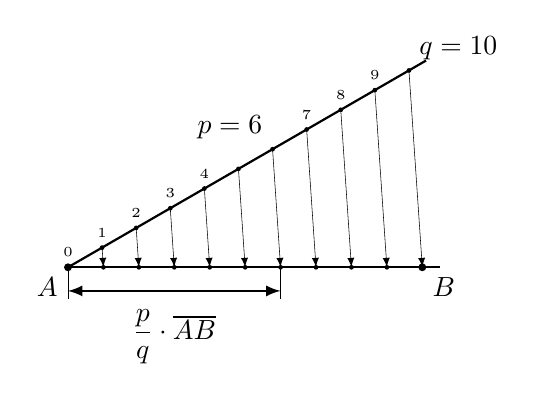
\begin{tikzpicture}[>=latex,thick]
\def\s{0.5}
\def\t{0.45}

\coordinate (A) at (0,0);
\coordinate (B) at ({10*\t},0);

\uncover<2->{
	\draw (0,0) -- (30:{10.5*\s});
}

\uncover<3->{
	\foreach \x in {0,...,10}{
		\fill (30:{\x*\s}) circle[radius=0.03];
	}
	\foreach \x in {0,1,2,3,4,7,8,9}{
		\node at (30:{\x*\s}) [above] {\tiny $\x$};
	}
	\node at (30:{10*\s}) [above right] {$q=10$};
}

\uncover<4->{
	\foreach \x in {1,...,10}{
		\fill (0:{\x*\t}) circle[radius=0.03];
		\draw[->,line width=0.2pt] (30:{\x*\s}) -- (0:{\x*\t});
	}
}

\draw (A) -- (0:{10.5*\t});
\node at (A) [below left] {$A$};
\node at (B) [below right] {$B$};
\fill (A) circle[radius=0.05];
\fill (B) circle[radius=0.05];

\uncover<5->{
	\node at (30:{6*\s}) [above left] {$p=6$};
	\draw[line width=0.2pt] (0,0) -- (0,-0.4);
	\draw[line width=0.2pt] ({6*\t},0) -- ({6*\t},-0.4);
	\draw[<->] (0,-0.3) -- ({6*\t},-0.3);
	\node at ({3*\t},-0.4) [below]
		{$\displaystyle\frac{p}{q}\cdot\overline{AB}$};
}

\end{tikzpicture}
\end{center}
\end{column}
\begin{column}{0.48\textwidth}
\uncover<8->{%
\begin{center}
\begin{tikzpicture}[>=latex,thick]

%\foreach \x in {8,...,14}{
%	\only<\x>{\node at (4,4) {$\x$};}
%}

\def\r{4}
\def\a{50}

\coordinate (A) at ({\r*cos(\a)},0);

\uncover<10->{
	\fill[color=gray] (\r,0) -- (\r,0.3) arc (90:180:0.3) -- cycle;
	\fill[color=gray]
		(95:\r) -- ($(95:\r)+(185:0.3)$) arc (185:275:0.3) -- cycle;
}

\draw[->] (0,0) -- (95:\r);
\node at (95:{0.5*\r}) [left] {$c$};

\begin{scope}
	\clip (-1,-0.3) rectangle (4.5,4.1);
	\uncover<10->{
		\draw (-1,0) -- (5,0);
		\draw[->] (0,0) -- (\r,0);
		\draw (0,0) circle[radius=\r];
		\draw ({\r*cos(\a)},-1) -- ({\r*cos(\a)},5);
	}
\end{scope}

\uncover<11->{
	\fill[color=blue!20] (0,0) -- (A) -- (\a:\r) -- cycle;
}

\uncover<9->{
	\fill[color=gray!80] (A) -- ($(A)+(0,0.5)$) arc (90:180:0.5) -- cycle;
	\fill[color=gray!120] ($(A)+(-0.2,0.2)$) circle[radius=0.07];
	\draw ({\r*cos(\a)},-0.3) -- ({\r*cos(\a)},4.1);
}

\uncover<11->{
	\draw[color=blue,line width=1.4pt] (0,0) -- (\a:\r);
	\node[color=blue] at (\a:{0.5*\r}) [above left] {$c$};
}

\draw[color=blue,line width=1.4pt] (0,0) -- ({\r*cos(\a)},0);
\fill[color=blue] (0,0) circle[radius=0.04];
\fill[color=blue] (A) circle[radius=0.04];
\node[color=blue] at ({0.5*\r*cos(\a)},0) [below] {$a$};

\uncover<12->{
	\fill[color=white,opacity=0.8]
		({\r*cos(\a)+0.1},{0.5*\r*sin(\a)-0.25})
		rectangle
		({\r*cos(\a)+2},{0.5*\r*sin(\a)+0.25});

	\node[color=red] at ({\r*cos(\a)},{0.5*\r*sin(\a)}) [right]
		{$b=\sqrt{c^2-a^2}$};
	\draw[color=red,line width=1.4pt] ({\r*cos(\a)},0) -- (\a:\r);
	\fill[color=red] (\a:\r) circle[radius=0.05];
	\fill[color=red] (A) circle[radius=0.05];
}

\end{tikzpicture}
\end{center}}
\end{column}
\end{columns}
\uncover<14->{{\usebeamercolor[fg]{title}Folgerung:}
Konstruierbar sind Körpererweiterungen $[F:E] = 2^l$}
\end{frame}
